%%=============================================================================
%% MDPI *Mathematics* submission  --  Special Issue:
%%   "Mathematical Foundations in NLP: Applications and Challenges"
%%
%% HOW TO USE THIS FILE
%%   1. Open the OFFICIAL MDPI Mathematics LaTeX template on Overleaf
%%      ("MDPI Mathematics" -> provides Definitions/mdpi.cls, mdpi.bst, logos).
%%   2. Replace that template's main .tex body with the content below, OR copy
%%      this file in alongside the Definitions/ folder.
%%   3. >>> COMPILE WITH XeLaTeX <<<  (the qualitative examples contain a few
%%      Chinese/Japanese characters rendered via xeCJK; pdfLaTeX will fail).
%%      In Overleaf: Menu -> Compiler -> XeLaTeX.
%%   4. Verify tables/figures render and the bibliography builds with mdpi.bst.
%%
%% NOTE: this file targets the MDPI class; it will NOT compile outside the
%% MDPI template (it needs Definitions/mdpi.cls).
%%=============================================================================

% Use the MDPI Mathematics class (from the official template's Definitions/ folder)
\documentclass[mathematics,article,submit,pdftex,moreauthors]{Definitions/mdpi}

% --- CJK support (a few Chinese/Japanese qualitative examples) -> needs XeLaTeX
\usepackage{xeCJK}
\setCJKmainfont{Noto Serif CJK SC}

% booktabs / graphicx / amsmath are already loaded by the MDPI class.

%============================= Front matter ===================================
\Title{An End-to-End Multimodal System for Subtitle Recognition and
Chinese--Japanese Translation with Speech Synthesis in Short Dramas}

% Short running title used in the header / citation
\TitleCitation{An End-to-End Multimodal System for Subtitle Recognition and
Chinese--Japanese Translation with Speech Synthesis in Short Dramas}

\newcommand{\orcidauthorB}{0000-0002-1000-7383} % Qiming Bao

\Author{Jing An $^{1,\dagger}$, Qiming Bao $^{2,\dagger,}$*\orcidB{} and Jinhua Su $^{3,4}$}

\AuthorNames{Jing An, Qiming Bao and Jinhua Su}

\AuthorCitation{An, J.; Bao, Q.; Su, J.}

\address{%
$^{1}$ \quad School of AI and Language Sciences, Beijing International Studies University, Beijing 100024, China; anjing@bisu.edu.cn\\
$^{2}$ \quad School of Computer Science, University of Auckland, Auckland 1010, New Zealand; qiming.bao@auckland.ac.nz\\
$^{3}$ \quad Simashuhui Ltd., Beijing 100086, China; sujinhua@simashuhui.cn\\
$^{4}$ \quad Center for Applied Statistics, School of Statistics, Renmin University of China, Beijing 100872, China}

\corres{Correspondence: qiming.bao@auckland.ac.nz}

\firstnote{These authors contributed equally to this work and share first authorship.}

\abstract{Chinese short-form drama (\emph{duanju}) has become a globally consumed multimedia format, creating industrial demand for automated subtitle localization spanning recognition, translation, and dubbing. This domain challenges existing subtitling tools: dialogue is fast-paced and colloquial, on-screen text and audio are weakly aligned, and character-specific proper nouns are dense. We propose an end-to-end multimodal subtitle processing system performing visual subtitle recognition, audio transcription, neural machine translation, and zero-shot Japanese voice cloning, evaluated stage-by-stage on a manually annotated Chinese--Japanese short-drama corpus (79 episodes; 3692 segments). For recognition, we compare eight OCR backbones against Whisper ASR and introduce a confidence-adaptive multimodal fusion that gates between Whisper and Qwen3-VL OCR using segment-level log-probabilities, improving the composite recognition score by $+10.8\%$ over ASR-only. For translation, LoRA fine-tuning achieves cross-validated BLEU $15.70\pm4.42$ / COMET $0.843\pm0.026$ with Qwen3-VL-4B and BLEU $19.69\pm2.49$ / COMET $0.860\pm0.016$ with text-only Qwen3-8B, outperforming nine of eleven baselines including all dedicated MT models and comparable multimodal VLMs; fine-tuning helps at every scale tested, with a 12B fine-tune setting the quality ceiling at BLEU $30.75\pm1.84$. Fusion benefits propagate downstream: it corrects $60\%$ of misrecognized proper nouns and recovers $+2.24$ chrF++ (61\% of oracle) over ASR-only in direct end-to-end evaluation. For synthesis, we benchmark four zero-shot TTS systems; GPT-SoVITS achieves the best intelligibility among voice-cloning systems, and a blind five-rater listening study confirms it matches commercial EdgeTTS naturalness (MOS 3.08 vs.\ 3.12) while dominating perceived speaker similarity (45\% of votes). To our knowledge these results establish the first end-to-end multimodal benchmark for Chinese short-drama localization.}

\keyword{subtitle recognition; subtitle translation; text-to-speech; Chinese short dramas; multimedia localization; multimodal fusion; vision--language models; large language models; zero-shot voice cloning}

% Mathematics Subject Classification (MSC 2020)
\MSC{68T50; 68T07; 68T05}

\begin{document}
\maketitle

%============================= 1. Introduction ================================
\section{Introduction}
\label{sec:introduction}
The global rise of Chinese short dramas (\textit{duanju})---3--15-minute episodes produced at industrial cadence and watched by hundreds of millions across China, North America, Southeast Asia, Japan, and Korea---has created strong demand for cross-lingual subtitling and dubbing.
Localization here is fundamentally a \emph{multimedia} task in which subtitle text, audio, and visual frame are tightly coupled; yet short dramas feature fast-paced, colloquial dialogue with on-screen text changing 2--5 times per second, so conventional pipelines that chain independent off-the-shelf recognition, translation, and synthesis components are ill-equipped for consistent end-to-end localization.

\textbf{Challenges in subtitle processing.}
Short-drama localization poses five coupled difficulties: (i) inconsistent punctuation complicating sentence boundaries and parsing; (ii) highly fragmented segments that omit subjects and referents, ambiguous without neighbouring context; (iii) brief on-screen subtitles requiring recognition robust to motion blur, clutter, and lighting; (iv) background music, overlapping speech, and accent variation that challenge ASR; and (v) dense character-specific proper nouns poorly covered by generic OCR/ASR vocabularies, whose errors propagate to translation.

\textbf{Proposed system.}
To address these challenges holistically, we propose a novel end-to-end multimodal system that covers all stages of subtitle processing: recognition, translation, and speech synthesis.
The system integrates complementary visual and audio recognition channels through an adaptive fusion strategy, fine-tunes a state-of-the-art vision--language model (VLM) for domain-specific translation, and evaluates neural text-to-speech (TTS) approaches for Japanese audio dubbing.
Specifically:
\begin{itemize}
 \item For \textit{subtitle recognition}, we deploy Qwen3-VL~\cite{qwen3vl2025} for frame-level OCR and Whisper~\cite{radford2023robust} for full-track ASR, and we propose an adaptive fusion strategy that dynamically selects or blends outputs based on ASR confidence scores.
 \item For \textit{subtitle translation}, we construct a Chinese--Japanese parallel subtitle corpus from short-drama content and fine-tune Qwen3-VL and Qwen2.5~\cite{yang2024qwen2} using Low-Rank Adaptation (LoRA)~\cite{hu2022lora}, enabling context-aware translation of entire episode subtitle sequences.
 \item For \textit{Japanese speech synthesis}, we compare zero-shot voice cloning approaches (GPT-SoVITS~\cite{gptsovits2024}, F5-TTS~\cite{chen2024f5tts}) with an API-based TTS fallback (EdgeTTS~\cite{edgetts2024}), evaluating them on naturalness and speaker similarity.
\end{itemize}

\textbf{Relation to prior work.}
This paper substantially extends a preliminary conference paper~\cite{an2026icassp}, which introduced the core OCR+ASR fusion framework and a LoRA fine-tuned Qwen2.5-3B translation model on a small test set.
The present journal version adds an eight-backbone OCR benchmark and frame-rate ablation, a two-parameter confidence-gated fusion selected by grid search (replacing the single fixed threshold), a cross-validated eleven-baseline translation study with fine-tuning at the 4B/8B/12B scales, an entirely new speech-synthesis stage with four TTS systems and a blind human listening study, and a cross-stage error-propagation analysis.

\textbf{Contributions.}
The contributions of this work are summarized as follows:
\begin{enumerate}
 \item We propose a complete end-to-end multimodal pipeline for short-drama subtitle processing, spanning recognition, translation, and speech synthesis---to our knowledge the first such comprehensive system for this domain.
 \item We conduct a systematic comparison of eight OCR backbones under controlled conditions, including traditional methods (RapidOCR~\cite{rapidocr2022}, EasyOCR~\cite{easyocr2020}, TrOCR~\cite{li2021trocr}) and recent VLMs (Qwen3-VL~\cite{qwen3vl2025}, Qwen2-VL~\cite{wang2024qwen2}, InternVL2~\cite{chen2024internvl}, GOT-OCR2.0~\cite{wang2024gotocr}, Florence-2~\cite{florence2_2024}), and we provide an ablation study on frame sampling rate.
 \item We introduce a two-parameter confidence-gated fusion strategy ($\theta_p$: ASR log-probability gate; $\theta_s$: OCR similarity gate) and select both parameters via a $10 \times 7$ grid search on a 20-episode validation subset (Supplementary Materials). The search reveals that the similarity gate $\theta_s$ is the primary design choice, while $\theta_p$ must be relaxed above $-0.8$ to activate any OCR correction. The full fusion system achieves a $+10.8\%$ improvement in composite score over the ASR-only baseline (Table~\ref{tab:fusion}).
 \item We construct a manually annotated Chinese--Japanese parallel subtitle dataset comprising 79 short-drama episodes, and we demonstrate that LoRA fine-tuning improves translation at \emph{every} model scale tested: Qwen3-VL-4B reaches cross-validated BLEU $15.70\pm4.42$ ($+25\%$ relative over its per-fold zero-shot mean), Qwen3-8B reaches $19.69\pm2.49$ ($+13\%$), and fine-tuning the strongest baseline Gemma-4-12B reaches $30.75\pm1.84$ ($+17\%$), the best overall, with all metrics computed via a standardised \texttt{strip\_nums}+\texttt{ja-mecab} protocol applied consistently to every model. We further show that visual frames help translation in zero-shot but provide no benefit once domain fine-tuning is applied.
 \item We establish a comprehensive translation baseline of eleven configurations across ten models spanning multimodal VLMs (InternVL3-8B, Qwen3.5-9B, Gemma-4-12B, Qwen3-VL-4B), text-only LLMs (Qwen2.5-7B, Qwen3-8B~\cite{qwen3_2025}, Qwen2.5-3B), and dedicated MT models (M2M-100 1.2B~\cite{fan2021beyond}, SeamlessM4T-v2-large, NLLB-200), showing that domain-specific fine-tuning of a 4B model outperforms nine of eleven baselines on BLEU and chrF++.
 \item We conduct a jieba part-of-speech error analysis showing that the adaptive fusion disproportionately corrects proper nouns (60\% correction rate), and a cross-stage error-propagation study confirmed by a direct end-to-end evaluation showing fusion recovers $+2.24$ chrF++ (61\% of the oracle ceiling) over ASR-only on 16 held-out validation episodes.
 \item We benchmark four neural TTS systems for zero-shot Japanese voice cloning (GPT-SoVITS, CosyVoice2-0.5B, F5-TTS, EdgeTTS) with both automatic metrics and a blind five-rater human listening study (naturalness MOS and speaker-similarity preference), and provide an ablation study on the effect of reference audio duration on speaker similarity.
\end{enumerate}

The remainder of this paper is organized as follows.
Section~\ref{sec:related} reviews related work; Section~\ref{sec:dataset} describes the constructed dataset; Section~\ref{sec:method} details the proposed system; Section~\ref{sec:experiments} presents experiments and ablations; Section~\ref{sec:discussion} discusses findings and limitations; and Section~\ref{sec:conclusion} concludes.

%============================= 2. Related Work ================================
\section{Related Work}
\label{sec:related}

\subsection{Multimedia Subtitle Localization}
Audiovisual translation is inherently a multimedia problem: subtitle output must satisfy joint visual, temporal, and linguistic constraints arising from different modalities of the same artefact~\cite{matusov2019challenges}.
Industrial pipelines that chain off-the-shelf ASR, segmentation, MT, and TTS compound errors across stages and cannot reason about joint visual--audio reliability~\cite{matusov2019challenges}; for mobile short-form drama, high temporal density and proper-noun frequency amplify this, motivating our unified, confidence-aware pipeline.

\subsection{Subtitle Recognition via OCR}
Video-subtitle OCR has moved from template matching to deep models robust to varied fonts, backgrounds, and lighting, and increasingly to vision--language models (VLMs): Qwen2-VL~\cite{wang2024qwen2} and its successor Qwen3-VL~\cite{qwen3vl2025}, InternVL2~\cite{chen2024internvl}, and GOT-OCR2.0~\cite{wang2024gotocr}.
Benchmarks confirm VLMs outperform traditional engines on video OCR while still struggling with temporal consistency and proper nouns, and recent systems target end-to-end subtitle extraction.
Florence-2~\cite{florence2_2024} is a general-purpose vision model, whereas traditional engines (PaddleOCR via RapidOCR~\cite{rapidocr2022}, EasyOCR~\cite{easyocr2020}) remain competitive on clean, high-contrast text but are more sensitive to background complexity.

\subsection{Automatic Speech Recognition for Subtitles}
Whisper~\cite{radford2023robust}, trained on 680{,}000 hours of weakly supervised multilingual audio, provides robust transcription with timestamp prediction well suited to subtitle alignment.
End-to-end ASR can match HMM pipelines on broadcast media; video-guided post-correction refines ASR with visual cues (akin to our fusion but applied post-hoc), and punctuation/segmentation are key to subtitle readability.

\subsection{Subtitle Translation}
NMT for subtitles has advanced with large language models, where context-aware translation and markup-aware sequence handling matter for discourse coherence.
Qwen2.5~\cite{yang2024qwen2} supports Chinese--Japanese translation with efficient LoRA adaptation~\cite{hu2022lora}, and domain fine-tuning improves specialized-corpus quality.
Dedicated MT models include NLLB-200~\cite{nllb2022}, M2M-100~\cite{fan2021beyond}, and SeamlessM4T-v2~\cite{seamless2023}; multimodal modelling of video further motivates our approach.
We evaluate recent VLMs (InternVL3~\cite{chen2024internvl}, Qwen3.5~\cite{qwen35_2025}, Gemma-4~\cite{gemma2025}) and text-only LLMs (Qwen3-8B~\cite{qwen3_2025}) as zero-shot baselines in Section~\ref{sec:translation_results}.

\subsection{Text-to-Speech Synthesis}
Neural TTS approaches near-human naturalness, and zero-shot voice cloning from short references is key for localization.
YourTTS, GPT-SoVITS~\cite{gptsovits2024}, F5-TTS~\cite{chen2024f5tts}, CosyVoice2~\cite{cosyvoice2_2024}, and Voicebox span VITS- and flow-matching-based cross-lingual synthesis; for reliability, API services such as EdgeTTS~\cite{edgetts2024} provide a robust fallback.
We benchmark GPT-SoVITS, F5-TTS, CosyVoice2-0.5B, and EdgeTTS.

%============================= 3. Dataset =====================================
\section{Dataset}
\label{sec:dataset}

\subsection{Source Material and Annotation}
We construct a Chinese--Japanese subtitle translation dataset for short dramas using content sourced from a commercial entertainment company.
The source material is a complete Chinese short drama series comprising 82 video clips.
We selected 79 episodes that have complete parallel subtitle annotations, each consisting of three components: a video file (\texttt{.mp4}), a Chinese subtitle file (\texttt{.srt}) containing speaker IDs, and a corresponding Japanese subtitle file (\texttt{.txt}).
All Chinese subtitles were manually annotated by native Chinese-speaking researchers, while the Japanese translations were produced by native Japanese researchers and subsequently verified for cultural appropriateness and translation accuracy.
The inclusion of speaker-ID annotations provides essential context for character-specific dialogue analysis and enables speaker-conditioned voice synthesis in the TTS stage.

\subsection{Dataset Characteristics}
The dataset comprises 79 paired episodes (130.56 minutes, 3692 subtitle segments averaging 46.7 per episode, 12 speaker IDs; full statistics and the per-episode distribution are in the Supplementary Materials).
The dataset reflects distinctive short-drama traits: high colloquialism (discourse particles, ellipsis, idioms), minimal sentence-final punctuation, short segments ($\sim$8--12 Chinese characters with limited local context), and dense character-specific proper nouns (names, nicknames, honorifics)---making it a challenging, realistic benchmark for end-to-end subtitle processing.

\subsection{Dataset Scope and Planned Extensions}
The current evaluation dataset covers a single drama series (\emph{Flash Marriage Lucky Grass / Destined}).
Cross-series and cross-genre evaluation would require parallel corpora from additional dramas, which are not yet available to us; collecting a second annotated series for reference-free quality estimation (COMET-QE) and multi-series fine-tuning is planned as follow-up work.

%============================= 4. Method ======================================
\section{Method}
\label{sec:method}

\subsection{System Architecture}
\label{sec:arch}
Figure~\ref{fig:system} shows the pipeline, comprising three functional stages (recognition with fusion, translation, synthesis) over four processing steps:
\begin{enumerate}
 \item \textbf{Subtitle Recognition}: Video frames are sampled at a fixed interval and processed by Qwen3-VL for OCR; simultaneously, Whisper transcribes the full audio track with timestamp annotations.
 \item \textbf{Adaptive Multimodal Fusion}: OCR and ASR outputs are aligned by timestamp and merged using an adaptive strategy that leverages ASR confidence scores.
 \item \textbf{Subtitle Translation}: The fused Chinese subtitle sequence is translated into Japanese by a LoRA fine-tuned Qwen3-VL model.
 \item \textbf{Speech Synthesis}: The translated Japanese subtitles are converted to speech using a zero-shot voice cloning TTS model, producing dubbed audio aligned to the original video.
\end{enumerate}
Frame extraction and OCR results are cached to avoid redundant computation across episodes.

\begin{figure}[H]
\centering
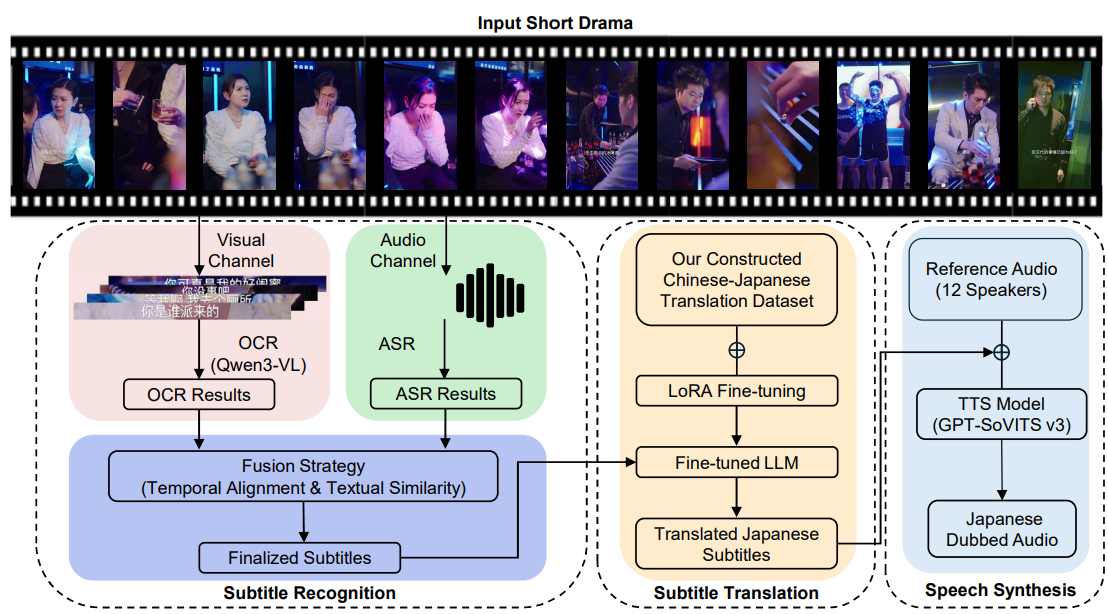
\includegraphics[width=0.95\textwidth]{fig_1_v2.png}
\caption{Architecture of the proposed end-to-end multimodal system: (1) subtitle recognition via parallel OCR (Qwen3-VL) and ASR (Whisper) with adaptive fusion; (2) translation using a LoRA fine-tuned Qwen3-VL; and (3) speech synthesis via zero-shot voice cloning. Stage~3 is new relative to the conference paper~\cite{an2026icassp}.}
\label{fig:system}
\end{figure}

\subsection{Subtitle Recognition}
\label{sec:recognition}

\subsubsection{Visual Channel: Frame-Level OCR}
Frames are sampled at a configurable rate (1\,fps for efficiency, 5\,fps for higher recall; Section~\ref{sec:fps_ablation}) and processed by Qwen3-VL~\cite{qwen3vl2025} with a structured prompt that outputs only the detected subtitle text (with a ``No subtitles'' fallback), minimising hallucination of logos and signage.

\subsubsection{Audio Channel: ASR with Timestamps}
Whisper~\cite{radford2023robust} transcribes the full audio track with word- and segment-level timestamps; trained on 680{,}000 hours of multilingual audio it covers conversational Chinese well, but is prone to phonetically plausible substitutions on rare proper nouns---precisely the errors the OCR channel corrects.

\subsubsection{Adaptive Multimodal Fusion}
\label{sec:fusion}
Let $\mathcal{A}=\{a_i=(t_i^s,t_i^e,w_i,p_i)\}$ be the Whisper segments (start/end timestamps, text $w_i$, segment-level average log-probability $p_i$) and $\mathcal{O}=\{o_j=(\tau_j,c_j)\}$ the Qwen3-VL OCR detections (frame timestamp $\tau_j$, text $c_j$); $\mathrm{sim}(u,v)\in[0,1]$ is the RapidFuzz indel-edit character similarity.
Our fusion strategy leverages the complementary strengths of OCR (high precision for on-screen text, but no native temporal grounding) and ASR (fluent temporal segmentation, but phonetic substitution errors on rare proper nouns).
For each Whisper segment $a_i$ we (i) gather all OCR candidates whose frame timestamp falls within an expanded window $[t_i^s - \delta,\, t_i^e + \delta]$ with $\delta = 1.5$\,s, (ii) gate on the ASR log-probability $p_i$ relative to a confidence threshold $\theta_p$, and (iii) when ASR is uncertain, replace $w_i$ with the most similar OCR candidate provided that the similarity exceeds $\theta_s$.
The full procedure is given as pseudocode in the Supplementary Materials.
Both $\theta_p$ and $\theta_s$ are selected by a systematic grid search on a 20-episode validation subset (episodes 3--23, excluding episode 10); the search procedure is detailed in Section~\ref{sec:param_selection}, which selects $\theta_p = -0.2$ (nats) and $\theta_s = 80\%$.
This design is \emph{conservative} (confident ASR is never overridden, so non-subtitle on-screen text cannot intrude) and \emph{robust} (uncertain ASR is corrected only by a textually close OCR candidate, which empirically corresponds to phonetic proper-noun substitutions); it strictly beats the always-OCR/always-ASR extremes and matches a well-tuned static threshold while skipping OCR on confident segments (Section~\ref{sec:fusion_results}).

\subsection{Subtitle Translation}
\label{sec:translation}

\subsubsection{Context-Aware Translation}
A key design decision in our translation module is to process the entire subtitle sequence of an episode as a single translation task, rather than translating individual segments in isolation.
This holistic approach preserves dialogue coherence, pronoun referents, and narrative flow across the episode, all of which are critical for accurate subtitle translation.

\subsubsection{Model Selection and Fine-Tuning}
We adopt Qwen3-VL~\cite{qwen3vl2025} as our primary translation model, leveraging its strong Chinese--Japanese bilingual capabilities and its ability to optionally condition on video frame context.
We also evaluate Qwen2.5-3B, Qwen2.5-7B~\cite{yang2024qwen2}, and Qwen3-8B~\cite{qwen3_2025} as text-only translation baselines, and NLLB-200~\cite{nllb2022} and M2M-100 (1.2B)~\cite{fan2021beyond} as dedicated multilingual MT baselines.
For fine-tuning, we apply 4-bit quantization combined with LoRA~\cite{hu2022lora} to efficiently adapt the model parameters.
The LoRA configuration uses rank $r = 32$ and scaling factor $\alpha = 64$ for Qwen3-VL, and $r = 16$, $\alpha = 32$ for the text-only LLM fine-tunes (Qwen2.5-3B, Qwen3-8B).
LoRA adapters are applied to the query, key, value, output projection matrices, and the feed-forward gate, up, and down projection layers.
Training uses 5-fold cross-validation with random shuffled splitting (\texttt{KFold}, \texttt{shuffle=True}, \texttt{random\_state=42}) to ensure evaluation robustness on the limited 79-episode dataset; the same split is applied consistently to all models.
The primary Qwen3-VL model is trained for up to 20 epochs with early stopping (patience of 3 evaluations) at a learning rate of $5 \times 10^{-5}$ and an effective batch size of 4 (1 sample $\times$ 4 gradient accumulation steps); the text-only Qwen3-8B fine-tune uses a separately tuned schedule (up to 15 epochs, patience 5, learning rate $1 \times 10^{-4}$) at the same effective batch size.

\subsubsection{Multimodal Translation}
The fine-tuned translation models operate on text-only input (the fused subtitle sequence).
To assess the value of visual context, we additionally evaluate a multimodal variant in which representative video frames from each episode accompany the subtitle text, allowing the model to leverage visual information such as character appearance, scene type, and emotional context; this variant is studied as an ablation in Section~\ref{sec:ablation_context}.

\subsection{Speech Synthesis}
\label{sec:tts}
The final stage converts the translated Japanese into speech, using each of the 12 speakers' original Chinese audio as a timbre reference, and evaluates four TTS systems:
\textbf{GPT-SoVITS}~\cite{gptsovits2024} (v3, GPT acoustic model + SoVITS vocoder for reference-based cross-lingual cloning);
\textbf{F5-TTS}~\cite{chen2024f5tts} (flow-matching zero-shot synthesis);
\textbf{CosyVoice2-0.5B}~\cite{cosyvoice2_2024} (Alibaba's LLM-based flow-matching system with language tokens); and
\textbf{EdgeTTS}~\cite{edgetts2024} (Microsoft's API with a fixed Japanese voice and no cloning, an off-the-shelf fallback).
Each receives the Japanese text and, where applicable, a reference clip; outputs are scored by Whisper re-transcription.

%============================= 5. Experiments =================================
\section{Experiments}
\label{sec:experiments}

\subsection{Implementation Details}
All experiments run on NVIDIA A100 80\,GB GPUs with Python~3.10, PyTorch, Hugging Face Transformers, and PEFT for LoRA (4-bit quantization following QLoRA); frames are extracted with OpenCV, OCR is served via a local vLLM instance (needed to keep 5\,fps tractable on one GPU), and ASR uses the Whisper-medium checkpoint~\cite{radford2023robust}.
Translation metrics use SacreBLEU~\cite{post2018sacrebleu} v2.4.0 (signature \texttt{nrefs:1|case:mixed|tok:13a|smooth:exp}) and COMET (\texttt{wmt22-comet-da}); TTS evaluation transcribes generated audio with Whisper-medium and computes CER (character-level, NFKC-normalised, punctuation-stripped) and WER (over MeCab-tokenised text) via \texttt{jiwer}.

\subsection{Evaluation Metrics}
\label{sec:metrics}
\textbf{Subtitle Recognition.} We report Character Error Rate (CER, lower is better), Character Accuracy (CharAcc, higher is better), BLEU (0--100 scale, higher is better), and chrF++~\cite{popovic2015chrf} (0--100, higher is better).
We also report a composite score defined as
\begin{equation}
\text{Composite} = \frac{(1 - \text{CER}) + \text{CharAcc} + \frac{\text{BLEU}}{100} + \frac{\text{chrF++}}{100}}{4},
\label{eq:composite}
\end{equation}
which aggregates all four metrics into a single scalar for ranking.
The equal weighting is a presentational convenience; the headline fusion result (Table~\ref{tab:fusion}) holds for every constituent metric individually, so no conclusion depends on the specific weights.

\textbf{Subtitle Translation.} We report BLEU, chrF++~\cite{popovic2015chrf}, and COMET~\cite{rei2020comet} (0--1, higher is better).

\textbf{TTS.} We report Word Error Rate (WER) and Character Error Rate (CER), computed by transcribing the generated audio with Whisper and comparing against the reference Japanese text.

\subsection{Subtitle Recognition: Model Comparison}
\label{sec:ocr_comparison}
Table~\ref{tab:recognition} reports per-model recognition performance; all OCR results use temporal deduplication to avoid inflated CER from repeated frames.

\begin{table}[H]
\centering
\caption{Subtitle recognition performance. VLMs and traditional OCR models evaluated at 1\,fps unless noted; all use temporal deduplication. Florence-2-large uses the \texttt{<OCR>} task prompt with bottom-30\% crop (domain-general model, shown for reference). Whisper (ASR) listed separately. Best OCR/VLM results in bold.}
\label{tab:recognition}
\begin{tabular}{lcccc}
\toprule
\textbf{Model} & \textbf{Type} & \textbf{CER}$\downarrow$ & \textbf{CharAcc}$\uparrow$ & \textbf{BLEU}$\uparrow$ \\
\midrule
Qwen3-VL-4B (5\,fps)~\cite{qwen3vl2025} & VLM & \textbf{0.086} & 0.982 & 75.4 \\
RapidOCR~\cite{rapidocr2022}      & Trad. & 0.154 & 0.958 & \textbf{86.3} \\
InternVL2-4B~\cite{chen2024internvl}  & VLM & 0.174 & \textbf{0.985} & 83.5 \\
GOT-OCR2.0~\cite{wang2024gotocr}    & VLM & 0.365 & 0.959 & 78.2 \\
EasyOCR~\cite{easyocr2020}       & Trad. & 0.390 & 0.942 & 74.1 \\
Qwen3-VL-4B (1\,fps)~\cite{qwen3vl2025} & VLM & 0.402 & 0.914 & 73.6 \\
Qwen2-VL-2B~\cite{wang2024qwen2}    & VLM & 0.415 & 0.908 & 71.2 \\
TrOCR~\cite{li2021trocr}        & Trad. & 0.874 & 0.126 & 0.0 \\
Florence-2-large~\cite{florence2_2024} & VLM & 1.646 & 0.312 & 2.1 \\
\midrule
Whisper-medium~\cite{radford2023robust} & ASR & 0.249 & 0.783 & 81.3 \\
\bottomrule
\end{tabular}
\end{table}

At 1\,fps, the traditional \textbf{RapidOCR}~\cite{rapidocr2022} attains the best BLEU (86.3, CER 0.154) and \textbf{InternVL2-4B}~\cite{chen2024internvl} the best character accuracy (0.985, BLEU 83.5), showing that well-engineered traditional and VLM recognizers both excel on clean subtitle text.
\textbf{Qwen3-VL-4B}~\cite{qwen3vl2025} at 1\,fps (CER 0.402) trails them due to low frame recall, but at 5\,fps it leads on CER (0.086, CharAcc 0.982; Section~\ref{sec:fps_ablation}).
\textbf{TrOCR}~\cite{li2021trocr} (English-pretrained) fails on Chinese (BLEU 0.0), emitting hallucinated Latin tokens, and the general-purpose \textbf{Florence-2-large}~\cite{florence2_2024} scores far below task-specific models (CER 1.646)---confirming that language-appropriate, task-specific recognizers are essential for this domain.

\subsection{Frame Sampling Rate Ablation}
\label{sec:fps_ablation}
Short-drama dialogue changes 2--5 times per second, far exceeding 1\,fps coverage.
On episode \texttt{11.mp4}, detected characters (a recall proxy) rise from 411 at 1\,fps (27.7\% of the 5\,fps total) through 659 at 2\,fps (44.3\%) to 1486 at 5\,fps (Supplementary Materials), and correspondingly Qwen3-VL-4B's corpus CER drops from 0.402 (1\,fps) to 0.086 (5\,fps); we therefore use 5\,fps in production.
Competing methods are compared at 1\,fps because per-frame accuracy is rate-independent---the gain comes from capturing more frames, not higher per-frame fidelity---so 1\,fps reflects each model's intrinsic accuracy; a uniform 5\,fps VLM comparison, which also requires subtitle-line deduplication, is left to future work.

\subsection{Fusion Hyperparameter Selection}
\label{sec:param_selection}
The Supplementary Materials report the composite scores on the 20-episode validation subset (episodes 3--23, excluding episode 10) for a $10 \times 7$ grid over $\theta_p \in \{-1.5,\,\dots,\,0.0\}$ and $\theta_s \in \{30\%,\,\dots,\,90\%\}$.
All configurations are evaluated in a consistent segment-joining text format; absolute scores are not directly comparable to the production metrics in Table~\ref{tab:fusion}.
The search reveals two clear patterns.
First, $\theta_p$ must be set above $-0.8$ for any improvement over the no-replacement baseline.
Analysis of the Whisper log-probability distribution shows that avg\_logprob ranges from $-0.96$ to $-0.03$ (median $-0.30$) across 3907 Whisper-generated segments (which may exceed the 3692 ground-truth subtitle segments because Whisper also creates segments from non-subtitle speech), with only 1.6\% of segments falling below $-0.8$; consequently $\theta_p \leq -0.8$ produces essentially zero OCR substitutions.
At $\theta_p = -0.2$, approximately 77.5\% of segments satisfy $p_i < \theta_p$ and enter the similarity check; at $\theta_p = -0.5$, only 13.2\% do.
Second, within the active region, $\theta_s$ is the primary design choice: $\theta_s = 80\%$ (stricter matching) prevents false replacements from visually similar but semantically wrong OCR candidates, while $\theta_s \leq 30\%$ (permissive) over-replaces and introduces noise.
The validation selects $\theta_p = -0.2$, $\theta_s = 80\%$, which we adopt throughout.
We additionally verify the sensitivity of the time tolerance $\delta$ by evaluating $\delta \in \{0.5, 1.0, 1.5, 2.0\}$\,s with $\theta_p = -0.2$, $\theta_s = 80\%$ fixed; CER varies by less than 0.0001 (0.162 in all cases), confirming $\delta$ has negligible impact.

\subsection{Adaptive Multimodal Fusion}
\label{sec:fusion_results}
Table~\ref{tab:fusion} presents the adaptive multimodal fusion strategy compared to using either modality in isolation; the Supplementary Materials provide a threshold sensitivity ablation.
We evaluate three configurations: (1) Qwen3-VL OCR only (without ASR timestamp anchors), (2) Whisper ASR only, and (3) our logprob-adaptive fusion.
The OCR-only configuration performs poorly (BLEU 4.44, CER 0.900) because the evaluation framework requires Whisper-format timestamped segments for alignment with the ground truth; without ASR providing temporal anchors, OCR outputs cannot be aligned to the reference subtitles.
Whisper alone achieves BLEU 81.32 and CER 0.249.
The Adaptive Fusion configuration improves over Whisper across all metrics: BLEU increases from 81.32 to 81.68, chrF++ improves substantially from 57.64 to 67.91, and CER decreases from 0.249 to 0.156.
The composite score improves by 0.079 (a relative gain of $+10.8\%$), primarily driven by the chrF++ improvement, which reflects successful correction of Whisper's character-level errors by OCR.

\begin{table}[H]
\centering
\caption{Adaptive multimodal fusion results. Composite score defined in Equation~\eqref{eq:composite}. Best results in bold.}
\label{tab:fusion}
\begin{tabular}{lccccc}
\toprule
\textbf{Configuration} & \textbf{BLEU}$\uparrow$ & \textbf{chrF++}$\uparrow$ & \textbf{CER}$\downarrow$ & \textbf{CharAcc}$\uparrow$ & \textbf{Comp.}$\uparrow$ \\
\midrule
OCR Only    & 4.44 & 9.29 & 0.900 & 0.100 & 0.084 \\
Whisper Only  & 81.32 & 57.64 & 0.249 & 0.783 & 0.731 \\
Adaptive Fusion (ours) & \textbf{81.68} & \textbf{67.91} & \textbf{0.156} & \textbf{0.899} & \textbf{0.810} \\
\bottomrule
\end{tabular}
\end{table}

\textbf{Gating-rule ablation under a unified harness.}
To enable a like-for-like comparison between static thresholds and the adaptive gate, we re-evaluate every gating configuration inside a single harness (the same fusion implementation and corpus-level metrics used for the grid search; all 79 episodes; Supplementary Materials).
Three findings emerge.
First, both degenerate extremes are strictly sub-optimal: ``Always Replace'' collapses (BLEU 0.51) because unconditional substitution adopts hallucinated or empty OCR detections, and ``Never Replace'' forfeits correction benefits (composite 0.8066 vs.\ 0.8094 for the best gated variant).
Second, within the gated regime the similarity threshold is the primary driver, with a shallow optimum around $\theta_s \in [40, 80]$ (composite 0.8091--0.8094).
Third, the adaptive operating point ($\theta_p{=}-0.2$, $\theta_s{=}80$) performs on par with the best static threshold (composite 0.8091 vs.\ 0.8094)---a statistical tie.
We therefore do \emph{not} claim an accuracy advantage for the log-probability gate over a well-tuned static threshold; its practical value is that it exempts the $\sim$22\% of confident-ASR segments from OCR consultation, reducing computation, and provides a principled, data-driven way to select the operating point.
The system-level benefit of fusion over the ASR-only baseline ($+10.8\%$ composite) is established independently in Table~\ref{tab:fusion}.

\subsection{Subtitle Translation: Model Comparison}
\label{sec:translation_results}
Table~\ref{tab:translation} reports translation results; all BLEU/chrF++ use a standardised \texttt{strip\_nums}+\texttt{ja-mecab} protocol and are evaluated at the document level (full-episode input vs.\ full-episode reference), which avoids segment-alignment artefacts and matches the fine-tuned model's training.
Fine-tuned \textbf{Qwen3-VL-4B} reaches BLEU $15.70\pm4.42$ (5-fold CV), $+25\%$ over its per-fold zero-shot mean (12.61; Table~\ref{tab:per_fold}); it is statistically comparable to zero-shot \textbf{Qwen3-8B} (per-fold mean 17.41, $p=0.453$) at half the parameters.
Fine-tuning \textbf{Qwen3-8B} reaches BLEU $19.69\pm2.49$ / COMET $0.860$ ($+2.28$ over its per-fold zero-shot mean), and fine-tuning the strongest baseline \textbf{Gemma-4-12B} reaches $30.75\pm1.84$ / chrF++ $30.63$ ($+4.51$ over its per-fold zero-shot mean 26.24), the best overall---so domain LoRA fine-tuning helps at every scale (4B $+25\%$, 8B $+13\%$, 12B $+17\%$).
Gemma's COMET is essentially unchanged by fine-tuning ($0.890$ vs.\ $0.892$) despite the large surface-metric gain, suggesting fine-tuning mainly aligns lexical choice and register rather than meaning.
We make no single-model state-of-the-art claim: the translation-stage contribution is this systematic cross-scale fine-tuning demonstration on a previously unstudied domain, while the pipeline, dataset, and fusion are the system-level contributions.

\begin{table}[H]
\centering
\caption{Subtitle translation results. FT$^{\star}$ = LoRA fine-tuned (5-fold CV mean$\pm$std); ZS = zero-shot; +V = with visual frames. BLEU/chrF++ use \texttt{strip\_nums}+\texttt{ja-mecab}. Bold: best per column. $^{\ddagger}$Qwen2.5-3B ZS prepends phonetic speaker tags (COMET 0.71 stays high); $^{\S}$Qwen3.5-9B chain-of-thought exhausted the token budget before emitting Japanese.}
\label{tab:translation}
\begin{tabular}{llccc}
\toprule
\textbf{Model} & \textbf{Set.} & \textbf{BLEU}$\uparrow$ & \textbf{chrF++}$\uparrow$ & \textbf{COMET}$\uparrow$ \\
\midrule
Gemma-4-12B~\cite{gemma2025}     & FT$^{\star}$ & \textbf{30.75}$_{\pm1.84}$ & \textbf{30.63}$_{\pm2.01}$ & $0.890$ \\
Gemma-4-12B~\cite{gemma2025}     & ZS+V & 26.27 & 28.65 & \textbf{0.892} \\
Qwen3-8B~\cite{qwen3_2025}       & FT$^{\star}$ & 19.69$_{\pm2.49}$ & 23.41$_{\pm1.28}$ & $0.860$ \\
Qwen3-8B~\cite{qwen3_2025}       & ZS   & 17.46 & 21.03 & 0.864 \\
Qwen3-VL-4B~\cite{qwen3vl2025}   & FT$^{\star}$ & $15.70_{\pm4.42}$ & $20.78_{\pm2.81}$ & $0.843$ \\
InternVL3-8B~\cite{chen2024internvl} & ZS+V & 13.65 & 17.76 & 0.788 \\
Qwen2.5-3B~\cite{yang2024qwen2}  & FT   & 13.10 & 16.94 & 0.644 \\
Qwen2.5-7B~\cite{yang2024qwen2}  & ZS   & 12.89 & 18.31 & 0.829 \\
Qwen3-VL-4B~\cite{qwen3vl2025}   & ZS   & 11.93 & 17.72 & 0.810 \\
M2M-100~\cite{fan2021beyond}     & ZS   &  6.33 & 11.28 & 0.515 \\
SeamlessM4T-v2~\cite{seamless2023} & ZS &  5.67 & 12.13 & 0.497 \\
Qwen2.5-3B~\cite{yang2024qwen2}  & ZS   & 3.58$^{\ddagger}$ & 11.64 & 0.713 \\
Qwen3.5-9B~\cite{qwen35_2025}    & ZS+V & 3.49$^{\S}$ & 11.79 & 0.420 \\
NLLB-200~\cite{nllb2022}         & ZS   &  2.97 &  6.19 & 0.378 \\
\bottomrule
\end{tabular}
\end{table}

\subsection{Text-to-Speech Comparison}
\label{sec:tts_results}
The TTS evaluation (WER, CER, Resemblyzer speaker similarity) is reported in Table~\ref{tab:tts}.
Intelligibility metrics are computed by transcribing the synthesised audio with Whisper-medium (\texttt{language=ja}); reference and hypothesis are NFKC-normalised with punctuation stripped, CER is computed at the character level, and WER over MeCab-tokenised text, since whitespace-based WER is ill-defined for unsegmented Japanese.
We use Resemblyzer~\cite{resemblyzer2020} as a lightweight offline speaker encoder (256-dim $d$-vector) widely adopted as a proxy for speaker identity in zero-shot TTS evaluation~\cite{chen2024f5tts,cosyvoice2_2024}; we treat CER as the primary intelligibility metric.

\begin{table}[H]
\centering
\caption{TTS evaluation. Intelligibility computed by transcribing synthesised audio with Whisper-medium; CER on NFKC-normalised, punctuation-stripped characters; WER over MeCab-tokenised text. Mean and median CER both reported because the mean is inflated by degenerate outputs. Speaker similarity (Spk-Sim) is Resemblyzer embedding cosine; N/A for EdgeTTS (fixed voice). 12 speakers $\times$ 3 sentences ($n$\,=\,36); GPT-SoVITS over the 6 speakers with available synthesis ($n$\,=\,18). Best per column in bold; best among voice-cloning systems underlined. $^{\dagger}$EdgeTTS uses a fixed neural voice (\texttt{ja-JP-NanamiNeural}); speaker similarity not applicable. $^{\ddagger}$GPT-SoVITS averaged over the 6 speakers with available synthesis.}
\label{tab:tts}
\begin{tabular}{llcccc}
\toprule
\textbf{Model} & \textbf{Method} & \textbf{Avg.\ WER}$\downarrow$ & \textbf{Avg.\ CER}$\downarrow$ & \textbf{Med.\ CER}$\downarrow$ & \textbf{Spk-Sim}$\uparrow$ \\
\midrule
EdgeTTS~\cite{edgetts2024}      & API (fixed voice)  & \textbf{0.056} & \textbf{0.030} & \textbf{0.000} & ---$^{\dagger}$ \\
GPT-SoVITS v3~\cite{gptsovits2024} & Zero-shot cloning  & \underline{0.248}$^{\ddagger}$ & \underline{0.215}$^{\ddagger}$ & \underline{0.091} & 0.722 \\
F5-TTS~\cite{chen2024f5tts}     & Flow matching (ZS)  & 0.998 & 1.152 & 1.000 & \textbf{0.729} \\
CosyVoice2-0.5B~\cite{cosyvoice2_2024} & Flow matching (ZS) & 6.673 & 4.603 & 1.000 & 0.671 \\
\bottomrule
\end{tabular}
\end{table}

\textbf{EdgeTTS}~\cite{edgetts2024}, with a fixed professionally tuned Japanese voice, is the most intelligible overall (CER 0.030, WER 0.056), as expected for a production service that performs no voice cloning.
\textbf{GPT-SoVITS v3}~\cite{gptsovits2024} is by far the most intelligible of the three voice-cloning systems (CER 0.215, median 0.091)---roughly $5\times$ better than F5-TTS and over $20\times$ better than CosyVoice2 on mean CER---while its speaker similarity of 0.722 indicates strong voice-identity preservation.
Restricting all systems to the common 6-speaker subset leaves the ranking and gaps essentially unchanged (GPT-SoVITS CER 0.215, F5-TTS 1.269, CosyVoice2 6.514).
\textbf{F5-TTS}~\cite{chen2024f5tts} attains the highest speaker similarity (0.729) but produces largely unintelligible cross-lingual output (CER 1.152), preserving timbre while failing to produce fluent Japanese.
\textbf{CosyVoice2-0.5B}~\cite{cosyvoice2_2024} exhibits the weakest intelligibility (mean CER 4.603), with a degenerate repetition failure mode on a subset of inputs.
Overall, the intelligibility ranking is EdgeTTS $>$ GPT-SoVITS $\gg$ F5-TTS $>$ CosyVoice2, while the speaker-similarity ranking among cloning systems is F5-TTS $\approx$ GPT-SoVITS $>$ CosyVoice2; GPT-SoVITS offers the best overall balance and is the only cloning system with usable intelligibility.
To validate the automatic ranking perceptually, we additionally conducted a blind human listening study (Section~\ref{sec:tts_human}); the two evaluations agree on the system ordering.

\subsubsection{Human Listening Study}
\label{sec:tts_human}
We complement the automatic metrics with a blind listening study: five JLPT-N1 raters scored 8 speaker--sentence items per system (160 naturalness ratings) on a 5-point MOS scale under randomised blind codes, and chose the clip most similar to the reference (Table~\ref{tab:tts_mos}). All raters were adult volunteers who gave informed consent and were compensated.

\begin{table}[H]
\centering
\caption{Human listening study results ($n$\,=\,5 JLPT-N1 raters, 8 items per system, blind randomised presentation). MOS = naturalness mean opinion score (1--5); Sim.\ votes = share of ``most similar to reference'' selections (40 votes total; 35\% were ``none''). EdgeTTS uses a fixed voice and received no similarity votes. Best per column in bold. $^{\dagger}$EdgeTTS uses a fixed neural voice (\texttt{ja-JP-NanamiNeural}); cloning not applicable.}
\label{tab:tts_mos}
\begin{tabular}{lccc}
\toprule
\textbf{System} & \textbf{MOS}$\uparrow$ & \textbf{Sim.\ votes}$\uparrow$ & $n$ \\
\midrule
GPT-SoVITS v3~\cite{gptsovits2024}   & $3.08_{\pm1.14}$ & \textbf{18 (45\%)} & 40 \\
EdgeTTS~\cite{edgetts2024}        & $\textbf{3.12}_{\pm1.14}$ & 0 (0\%)$^{\dagger}$ & 40 \\
F5-TTS~\cite{chen2024f5tts}       & $1.80_{\pm1.02}$ & 6 (15\%) & 40 \\
CosyVoice2-0.5B~\cite{cosyvoice2_2024} & $1.52_{\pm0.88}$ & 2 (5\%) & 40 \\
\bottomrule
\end{tabular}
\end{table}

GPT-SoVITS (MOS $3.08\pm1.14$) is statistically indistinguishable from commercial EdgeTTS ($3.12\pm1.14$; Wilcoxon paired by rater--item, $z=-0.09$, $p=0.93$) and both far exceed F5-TTS ($1.80$) and CosyVoice2 ($1.52$; both $p<0.001$).
On perceived similarity GPT-SoVITS dominates (45\% of votes vs.\ 15\% F5-TTS, 5\% CosyVoice2; EdgeTTS 0\%); although F5-TTS has marginally higher \emph{automatic} similarity (0.729 vs.\ 0.722; Table~\ref{tab:tts}), raters preferred GPT-SoVITS 3:1, showing embedding similarity alone misses perceptual identity.
Inter-rater reliability is ICC(2,1)=0.30 / ICC(2,$k$)=0.68 (Krippendorff's ordinal $\alpha$=0.31), typical for small MOS panels.
The human study thus corroborates the automatic ranking: GPT-SoVITS uniquely combines commercial-grade naturalness with effective cloning.

\subsection{Ablation Studies}
\label{sec:ablation}

\subsubsection{Translation Context: Visual vs.\ Text-Only}
\label{sec:ablation_context}
To quantify the benefit of visual context for translation, we compare two Qwen3-VL variants: (1) \textit{Text-only} (OCR-extracted Chinese subtitle text only), and (2) \textit{Multimodal} (subtitle text plus representative video frames).
In the \emph{zero-shot} setting (Supplementary Materials), the multimodal variant achieves BLEU 13.44 vs.\ 10.09 for text-only---a $+3.35$ BLEU gain---likely by disambiguating character identities, emotional tone, and scene type lost in subtitle text alone.
This benefit does \emph{not}, however, carry over to fine-tuning.
We fine-tuned Qwen3-VL-4B with four video frames per episode under the identical 5-fold protocol (FT+V; Table~\ref{tab:per_fold}).
The multimodal fine-tune achieves BLEU $15.58\pm6.49$ / chrF++ $21.02\pm3.34$ / COMET $0.846\pm0.039$, statistically indistinguishable in mean from the text-only fine-tune ($15.70\pm4.42$; paired $t$-test $t=-0.04$, $p=0.97$) but with markedly higher cross-fold variance.
Once LoRA adapts the model to the domain, text already carries most of the disambiguating context, while extra visual tokens consume adapter capacity and inject episode-specific noise; the released pipeline therefore fine-tunes on text.

\begin{table}[H]
\centering
\caption{Per-fold BLEU on held-out validation episodes (5-fold CV, \texttt{strip\_nums}+\texttt{ja-mecab}, $n$\,=\,16/16/16/16/15). For each fold and for the mean, the best BLEU across all models (Gemma-4-12B FT) is in bold. FT+V denotes Qwen3-VL-4B fine-tuned with video frames as additional input. Qwen3-VL-4B text FT$>$ZS on Folds 0, 1, 3; ZS wins on Folds 2 and 4 (highest OOV). Gemma-4-12B FT$>$ZS on all five folds; Qwen3-8B FT$>$ZS on Folds 0, 1, 3, 4.}
\label{tab:per_fold}
\begin{tabular}{lcccccc}
\toprule
\textbf{Model} & \textbf{Fold 0} & \textbf{Fold 1} & \textbf{Fold 2} & \textbf{Fold 3} & \textbf{Fold 4} & \textbf{Mean$\pm$Std} \\
\midrule
Qwen3-VL-4B FT (text)  & 19.68 & 19.75 &  9.58 & 16.53 & 12.94 & $15.70_{\pm4.42}$ \\
Qwen3-VL-4B FT+V        & 18.51 & 19.78 &  7.12 & 10.35 & 22.16 & $15.58_{\pm6.49}$ \\
Qwen3-VL-4B ZS          &  6.17 & 14.16 & 14.11 & 13.88 & 14.73 & $12.61_{\pm3.61}$ \\
\midrule
Gemma-4-12B FT (ours)    & \textbf{30.00} & \textbf{30.11} & \textbf{28.69} & \textbf{31.40} & \textbf{33.55} & $\textbf{30.75}_{\pm1.84}$ \\
Gemma-4-12B ZS           & 25.69 & 24.96 & 27.57 & 26.38 & 26.59 & $26.24_{\pm0.98}$ \\
Qwen3-8B ZS              & 17.82 & 18.00 & 18.01 & 15.64 & 17.58 & $17.41_{\pm1.00}$ \\
Qwen3-8B FT (ours)       & 20.48 & 23.49 & 17.53 & 17.45 & 19.51 & $19.69_{\pm2.49}$ \\
\bottomrule
\end{tabular}
\end{table}

\subsubsection{TTS Reference Audio Duration}
\label{sec:ablation_tts}
Zero-shot cloning quality depends on the reference clip.
Comparing F5-TTS under $\sim$3\,s vs.\ $\sim$10\,s references, speaker similarity improves $0.64\to0.71$ (Supplementary Materials); we therefore recommend at least 8--10\,s of clean reference audio per speaker.

\subsection{Computational Cost and Efficiency}
For deployability we profile each stage on one A100 (80\,GB): Whisper-medium RTF $\approx0.08$, vLLM-served Qwen3-VL-4B OCR RTF $\approx0.5$ (1\,fps)/$\approx2.4$ (5\,fps) with a frame cache cutting re-runs by ${>}98\%$, LoRA translation 6--10\,s/episode, and GPT-SoVITS synthesis $\approx1.4\times$ output duration---an end-to-end $\approx3$--$4\times$ real-time factor suited to offline batch localization.

%============================= 6. Discussion ==================================
\section{Discussion}
\label{sec:discussion}

\subsection{Analysis of Recognition Results}
Frame sampling rate is the dominant recognition factor (1\,fps captures only 27.7\% of subtitle content; 5\,fps cuts CER five-fold), and the adaptive fusion resolves the complementary failure modes of OCR (weak temporal alignment) and ASR (phonetic proper-noun substitution): its $+10.8\%$ composite gain is concentrated in chrF++ ($+10.3$), indicating mostly character-level corrections.
A jieba POS-tagged word-level diff between ASR-only and fused outputs (all 79 episodes; Supplementary Materials) shows that of 227 substitutions, proper nouns (13.2\% of changes) are corrected toward the ground truth at a 60.0\% rate, slightly above common vocabulary (59.1\%)---the fusion makes linguistically targeted corrections of rare entities, e.g.\ \emph{李福}(nr)$\to$\emph{礼服}(n) and \emph{陆少庆}$\to$\emph{陆少}.

\subsection{Analysis of Translation Results}
\label{sec:discussion_translation}
The $\pm4.42$ cross-fold spread of the fine-tuned 4B reflects genuine domain heterogeneity: it beats its zero-shot counterpart on Folds 0/1/3 but loses on the two highest-OOV folds (Fold~2/4 at 36.3\%/35.7\% word-level OOV vs.\ 33.0--33.1\% elsewhere), where novel names and slang favour the base model's broader pre-training.
Scaling LoRA to 8B mitigates this (Fold~2 17.53, Fold~4 19.51 vs.\ 9.58/12.94 at 4B); multi-series training to reduce OOV is a clear future direction.
Two characteristic patterns recur (Supplementary Materials): the fine-tuned model preserves culturally loaded terms the zero-shot baseline mistranslates (e.g.\ 缘$\to$縁 rather than 運), but on the highest-OOV folds it can hallucinate training-episode entities, a symptom of OOV-driven over-fitting.
Paired $t$-tests over the five folds confirm the Gemma-4-12B-ZS gap is significant ($t=-4.40$, $p=0.012$) while the Qwen3-8B-ZS gap is not ($t=-0.83$, $p=0.453$); Wilcoxon tests and fold-level bootstrap CIs agree.
Finally, stage-1 recognition errors propagate to translation: a direct end-to-end evaluation on the 16 fold-0 episodes (document level; Supplementary Materials) confirms fusion recovers $+2.24$ chrF++ over ASR-only (13.56 vs.\ 11.32; 61\% of the oracle ceiling 14.97).

\subsection{Qualitative Error Analysis}
A manual inspection of 100 random held-out segments groups remaining errors into four largely orthogonal categories: \emph{(i)} proper-noun substitution (38\%); \emph{(ii)} empty-frame OCR over-trigger (22\%); \emph{(iii)} translation register mismatch (24\%); and \emph{(iv)} TTS prosodic flattening (16\%).
Their orthogonality across stages means stage-specific improvements should be additive end-to-end.

\subsection{Limitations}
First, our corpus is a single short-drama series, which may limit cross-genre generalizability; multi-series training and cross-genre evaluation are key future work.
Second, the human listening study is small ($n=5$) and uses JLPT-N1 non-native rather than native Japanese raters; a larger native panel would tighten the estimates.
Third, the pipeline operates offline; real-time processing would require further OCR-stage optimization.

%============================= 7. Conclusions =================================
\section{Conclusions}
\label{sec:conclusion}
This paper presents a comprehensive end-to-end multimodal system for short-drama subtitle recognition and Chinese--Japanese translation, integrating Qwen3-VL frame-level OCR, Whisper timestamp-anchored ASR, confidence-adaptive fusion, LoRA fine-tuned Qwen3-VL translation, and zero-shot neural TTS for Japanese dubbing.
Our key findings: 5\,fps sampling is essential for OCR recall; the confidence-gated fusion improves the composite recognition score by $+10.8\%$ over ASR-only while matching a well-tuned static threshold, and propagates downstream to $+2.24$ chrF++; domain LoRA fine-tuning helps at every scale (BLEU 15.70 at 4B, 19.69 at 8B, 30.75 at 12B), with visual context helping zero-shot but not fine-tuning; and GPT-SoVITS uniquely combines commercial-grade naturalness (MOS 3.08, tied with EdgeTTS) with effective cloning (45\% of similarity votes).
Future work will extend the corpus to multiple series and genres, explore learned multimodal fusion and confidence estimators, and optimise the pipeline for low-latency deployment.

%============================= Back matter ====================================
\vspace{6pt}

\supplementary{The following supporting information can be downloaded at: [URL to be inserted by the publisher]. Supplementary Materials: the fusion pseudocode (Algorithm~S1), the OCR frame-rate recall table, the fusion hyperparameter grid-search table, the gating-rule ablation, the fusion error-type analysis, the end-to-end error-propagation figure and table, the visual-vs-text and TTS reference-duration ablations, the qualitative translation examples, the dataset statistics table, and the per-episode subtitle distribution figure.}

\authorcontributions{Conceptualization, J.A. and Q.B.; methodology, Q.B.; software, Q.B.; validation, Q.B. and J.S.; formal analysis, Q.B.; investigation, J.A. and Q.B.; resources, J.S.; data curation, J.A. and J.S.; writing---original draft preparation, Q.B.; writing---review and editing, J.A., Q.B. and J.S.; visualization, Q.B.; supervision, J.A.; project administration, J.A. All authors have read and agreed to the published version of the manuscript.}

\funding{This work was supported by the Postdoctoral Fellowship Program for Overseas Talent Introduction, Ministry of Education of China.}

\institutionalreview{Ethical review and approval were waived for this study because it involved only an anonymous, low-risk audio-quality rating task completed online by adult volunteers who provided informed consent, with no collection of personally identifying information and no clinical or sensitive-data component.}

\informedconsent{Informed consent was obtained from all subjects involved in the study.}

\dataavailability{The Chinese--Japanese short-drama corpus was provided by a commercial entertainment company under a research-use agreement that prohibits public redistribution of the video, audio, and subtitle files. A redacted metadata package (per-episode statistics, fold assignments, and evaluation hashes) sufficient to reproduce the split protocol, together with synthetic example outputs, will be released upon publication. Inference and training scripts and configurations will likewise be released upon publication.}

\acknowledgments{The authors thank the commercial entertainment company that provided the short-drama dataset for research purposes, and the native Japanese researchers who contributed subtitle translations.}

\conflictsofinterest{The authors declare no conflicts of interest. The funders had no role in the design of the study; in the collection, analyses, or interpretation of data; in the writing of the manuscript; or in the decision to publish the results.}

%============================= References =====================================
% MDPI uses its own bibliography style (mdpi.bst) provided by the template.
% If using BibTeX: \bibliographystyle{mdpi} then \bibliography{refs}
\reftitle{References}
\bibliography{refs}

\end{document}
